\documentclass[12pt,a4paper]{report}
%%\documentclass[12pt,a4paper,twoside,openright,fleqn,MSc]{cusatmscthesis}
\renewcommand{\baselinestretch}{1.15}

\usepackage{dcolumn}
%\newcolumntype{.}{D{.}{.}{-1}}
\usepackage{bm}
\usepackage[colorlinks = true,
            linkcolor = red,
            urlcolor  = blue,
            citecolor = blue,
            pdftitle=Nav-Dissertion]{hyperref}

\usepackage{braket}
\usepackage{graphicx,epsfig,color,subfigure,sidecap,float}
\usepackage{amsmath}
\usepackage{lipsum}
\usepackage{wrapfig}
\usepackage[paperwidth=210mm,paperheight=297mm,centering,hmargin=3cm,vmargin=3cm]{geometry}
\usepackage{tcolorbox}
\setlength{\parskip}{1em}
%\usepackage{natbib}
%\usepackage{mathpazo}
%\usepackage{chancery}
%\usepackage{bookman}
%\usepackage{newcent}
%\usepackage{charter}

\usepackage[scaled=.9]{helvet}
%\usepackage{avant}
%\renewcommand{\familydefault}{\sfdefault}

%%\fontfamily{pzc}\fontsize{10}{12pt}\selectfont

%+Make Index
%\usepackage{makeidx}
%\makeindex
%-Make Index
\bibliographystyle{unsrt}
\usepackage{amssymb}
\usepackage{amstext}
\usepackage{amsmath}
\usepackage{graphicx}
\usepackage{makeidx}
\makeindex
% Title Page
\title{
	\huge Simulating Neutrino Oscillations in a Quantum Computer}
	\vspace{0.5cm}
\author{\large Navaneeth Krishnan M\\
	\small CUSAT, India.}
\begin{document}

\maketitle
\pagebreak	
\chapter*{Introduction}
\emph{“ Can physics be simulated by a universal computer? [...] the physical world is quantum mechanical, and therefore the proper problem is the simulation of quantum physics [...] the full description of quantum mechanics for a large a system with R particles [...] has too many variables, it cannot be simulated with a normal computer with a number of elements proportional to R [ ... but it can be simulated with ] quantum computer elements. [...] Can a quantum system be probabilistically simulated by a classical (probabilistic, I’d assume) universal computer? [...] If you take the computer to be the classical kind I’ve described so far [..] the answer is certainly, No! “} 
\begin{flushright}
-Richard P Feynman \cite{feynman82}\cite{nielsen}
\end{flushright}


The primary aim of any sort of simulation is to solve the differential equation that governs the dynamics of the system. One of the most simple example of such an equation is the Newtons equation of motion,
\begin{equation}
m\frac{d^{2}x}{dx} = F
\end{equation}
Generally, the initial state of the system would be input to the problem. Using simulations, one aims to predict the state of the system at a later time or position. The first step in doing any simulation is the encoding of state of system digitally, which more often involves some approximation. Using the encoding scheme, we have to prepare the initial state of system. Then one has to discretize the dynamical differential equation in space and time. Discretization should be done in such a way that the iterative application of a procedure should evolve the state from initial to final conditions. The accuracy of output state predicted by the simulator depends upon discretization length. Theoretically, as the length of discretization decreases the result would be more accurate. But while computing we need to consider other errors that can arise while decreasing the discretization length is taken. Thus often an optimum value of discretization length. Now, Why this approach works?. This works because the error is bounded and not considerably grows as the number of iterations increases. Further, only those system that can be efficiently described can be simulated efficiently. Thus there are systems where such an approach fails.\par
Now comes the question of whether we can simulate a quantum system using a classical simulator. The short answer is yes. But it should be noted that often such simulations are inefficient and fail when the number of particles in the system is very high.  When we analyse the problem of simulating a quantum system, for most of simple quantum systems, the evolution is governed by the time-independent Schrodinger equation. 
\begin{equation}
i\hbar \frac{d}{dt}\ket{\psi} = \hat{H} \ket{\psi}
\end{equation}
On the position basis, the above equation will be 
\begin{equation}
i\hbar\frac{\partial}{\partial t}\psi(x)= \left[ -\frac{\partial^{2}}{\partial x^{2}}+V(x)\right] \psi(x)
\end{equation}
Where $\braket{x|\psi} = \psi(x)$.\par
Assume that we wish to simulate a simple two-level system (Qubit) that obeys time-independent Schrodinger equation. For such as system, we have to solve two differential equation to simulate it. If it is a two-qubit system then there would be four equations and so on. Thus, a general system of n qubits $2^{n}$ differential equations must be solved to simulate it. This exponential explosion in the equation is unavoidable unless we employ some approximate methods like Monte Carlo methods \cite{monte} which considerably reduce the number of equations. Such classical stochastic methods would allow us to evaluate the phase-space integrals of many-body quantum systems in polynomial time. But these methods are efficient while the function being integrated does not change its sign. Thus while using such methods, sampling of the function is done in a relatively small number of points. For systems like fermionic or frustrated systems, the integrals encounter the problem of sampling with non-positive semi-definite functions (referred to as negative sign problem \cite{troyer}\cite{georgescu}) which cause an exponential increase in computation time as the number of particles increases. Thus in such systems, Monte Carlo methods are shown to be inefficient. Other than Monte Carlo methods, there are methods like Density Functional Theory (DFT) \cite{dft}, mean-field theories, Green function-based methods, many-body perturbation theories \cite{mbpt} etc. These methods also have its own limitations.

Richard P Feynman was one of the persons who put forward a solution to this problem. He said that \emph{“ Let the computer itself be built of quantum mechanical elements which obeys quantum mechanical laws “} \cite{feynman82}. Feynman realized that such a quantum system - which later called a quantum computer - would be able to handle the exponential explosion of parameters that happen while solving a large number of equations without using an exponentially large number of physical resources. Even though Feynman proposed such a radical idea, he was not aware of how to realise simulations in such controllable quantum systems. More than a decade later, it was Lloyd who showed that quantum computer could act as a universal quantum simulator \cite{lloyd}. Here the term “universal” is used in the sense that the same system can be used to simulate vastly different problems. Of course, one has to make adjustments in the algorithm according to problem. 

Even though the quantum computer was proposed to simulate quantum mechanics, its uses extend far beyond it. The past three decades have revealed the true power of a quantum computer. Nowadays quantum computing and quantum information itself a topic of research. Further, it became later clear that we don’t always need a quantum computer for implementing quantum simulations. For simulating a particular quantum system, we only need a simple quantum system that has similar time evolution. That is, simple quantum devices that mimic the time evolution of other quantum systems can be used as simulators. But the drawback of such an approach is that such a simulator would be problem-specific (not universal). On the bright side, such simple systems can be easily controlled and designed compared to sophisticated quantum computers.

Based on the approach, we can broadly classify the quantum simulations into kinds; Analog Quantum Simulation (AQS) and Digital Quantum Simulations (DQS). In DQS we use quantum computers as simulators. Here we encode the time evolution of the quantum system in a quantum circuit comprising qubits and quantum gates.  The circuit is designed in such a way that the output of the circuit gives the time evolved state of the system under study.  A similar but different approach is taken in Analog Quantum Simulations. In AQS, a simple quantum system that is controllable is created depending upon the problem. This system is designed in such a way that it would mimic the time evolution of the system under study. Thus in this approach, simulations are done using a simple quantum system as simulators.

In recent years, the field of quantum simulations has gained momentum. The sudden spike in interest is two folds. The first one is its wide range of application. For instance, quantum simulations can be used in condensed matter for studying many difficult problems like quantum phase transitions, high Tc superconductivity, quantum magnetism etc. Other potential applications include fields like high energy physics, nuclear physics, cosmology, quantum chemistry etc. The second factor that accelerated the growth of quantum simulations is the recent progress in the field of quantum technologies. Recent years have witnessed development in different types of realization of quantum computers. Nowadays quantum computers are publicly accessible. Quantum simulators which can be used to perform simulations repeatedly are now available. Technologies to maintain coherent control over the system and to perform measurements have matured enough to make it possible.

In near future, quantum simulations will become a prominent tool for research for a wide variety of fields. In this milieu, the study of quantum simulations holds importance. This was the motivation for us to conduct this study. Here we are interested in the digital quantum simulations of phenomena called Neutrino oscillation. We use the quantum computing services provided by IBM to carry out our simulations. The scheme for such a simulation was put forward by Arg\"uelles and jones in 2017 \cite{jones}. They have encoded neutrino oscillation into a quantum circuit. Time evolution of the qubits is done by applying unitary single and two-qubit gates. The exact scheme will be discussed in the following sections $\ref{sec4}$ $\ref{sec5}$. 

In nature, neutrinos are produced in three distinct flavours electron, muon and tau. Neutrinos are produced through weak interactions. As neutrino beam propagates from source to detector neutrino flavour oscillate between the three flavours. The first evidence of neutrino exhibit flavour oscillation from the famous Ray Davis Homestake experiment \cite{ray}.  He reported a deficit in the flux of solar neutrinos (electron neutrinos)  from the value predicted by the Standard model. He used a chlorine-based detector and obtained a flux that was three times less than that of the theoretical value.  This observation of Ray Davis later came to be known “Solar Neutrino Problem”. For the contributions in the field of astrophysics, Ray Davis was awarded the Nobel prize in Physics in 2002. 

Following the Homestake experiment, different sort of powerful detectors was set up and studied the problem. All the experiments confirmed the deficit of neutrinos in the solar flux. Ray Davis performed his experiment in the 1960s. Interestingly, the idea of neutrino oscillation was put forward by Pontecorvo in 1957 \cite{ponte57}. Thus one can say that solution existed even before the problem. But in Pontecorvo’s version neutrino-anti neutrino undergo oscillation. He put forward this theory in analogy with the neutral kaon mixing that was known way before. Although such oscillations do not occur in nature, this formed a key conceptual foundation in developing the theory for neutrino oscillation. The theory for neutrino flavour oscillation was put forward first by Maki, Nakagawa, Sakata in 1962 \cite{maki} which was later elaborated by Pontecorvo in 1967 \cite{ponte68}. The solar neutrino deficit observed only a year after that. The solar neutrino problem baffled scientists for a long time. It was the team of Canadian scientists lead by Arthur B McDonald in Sudurbary Neutrino Observatory (SNO) that put an end to the mystery. They experimentally verified that electron neutrino produced in the sun undergo flavour oscillations. The deficit in the number of electron neutrinos was because neutrinos undergo flavour change while travelling to Earth \cite{mcdonald}. At the same time, a group of Japanese scientist lead by Takaaki Kajita verified neutrino oscillation by studying atmospheric neutrinos. Atmospheric neutrinos were produced when cosmic rays hit the Earth’s atmosphere. When it travels to the Earths surface they undergo flavour oscillations. The team led by Kajita was able to detect these flavour oscillations. For the experimental verification of neutrino flavour oscillation, both Kaajita and McDonald was awarded the Nobel prize in physics in 2015.

The verification that neutrinos can undergo oscillations comes with great consequences. It was known that neutrinos can undergo flavour oscillation only if they have mass. But according to the Standard Model, neutrinos are massless. Thus the phenomenon of neutrino oscillation insists on the modification of the standard model. Even though there are some minimal extensions of the Standard model to accomodate neutrino masses, exact theory is unknown.  Neutrino oscillation experiments gives us mass squared splittings and mixing angles ( will discuss it later ). But till now the actual mass of the three neutrinos are still unknown. Thus the study of neutrino oscillation is a door to explore physics outside the standard model. 

In this work, we performed simulation of the time evolution of a neutrino flavour state. During such simulations we were able to observe neutrino flavour oscillations. But the application of DQS extends more than the temporal evolution of the state of the system. DQS can be used to obtain certain properties of a quantum system. It has been shown that using DQS we can estimate the eigenvalues of the operators including Hamiltonian of the system. For example, Abrams and Lloyd have put forward an algorithm to find eigenvalues and eigenvectors of Hamiltonian \cite{abrams}. They have proposed an algorithm that uses quantum fast Fourier transform to evaluate eigenvalues and eigenstates. Similarly, Aspuru-Guzik \emph{et al.} by applying a recursive phase estimation algorithm have calculated the molecular ground state energies of lithium hydride and water molecule \cite{aspuru}. It has been also shown that DQS can be used to compute the partition function of the system \cite{lidar}. Moreover, people have shown that classical physics can efficiently be simulated by quantum computers \cite{meyer}\cite{sinha}. 

Here we used the DQS of neutrino oscillation to study the entanglement between different neutrino flavours. Blasone \emph{et al.} through a series of papers \cite{blasone2008}\cite{blasone2009}\cite{blasone2010}\cite{blasone2014}, have proposed the existence of single particle entanglement in neutrinos. It was van Enk who proposed single particles can have entanglement \cite{vanenk2003}\cite{vanenk2005}\cite{vanenk2006}. He explained single particle entanglement in the context of single photons. Blasone \emph{et al.} extended these concepts into the case of neutrinos. They also provided scheme to quantify the degree of entanglement in the system. They used a measure called \emph{entanglement entropy} to quantify the entanglement. We applied their results in to our circuit and were able to accurately predict the entanglement dynamics of the system. 

This report is organized as follow. In the first chapter [\ref{sec1}], we provide a brief introduction to quantum simulations. Different types of approach for performing quantum simulations are discussed in this chapter. The second chapter [$\ref{sec2}$] is dedicated for the discussion of neutrino oscillation. In this section, we discuss the neutrino oscillation theory (both two flavour and three flavour case) relevant for performing quantum simulations. In the following chapter [$\ref{sec3}$], we discuss about the entanglement in the neutrino. Chapter $\ref{sec4}$ and Chapter $\ref{sec5}$ deals with the simulation of neutrino in a quantum computer. The scheme of performing such a simulation is given in the fifth chapter. The following chapter contains the results of the simulations performed. The conclusions and outlook is given in the concluding section.


\newpage
\thispagestyle{empty}
\mbox{}
\newpage
\chapter{Quantum Simulations: An Overview}\label{sec1}

Simulating a quantum system by quantum mechanical means is defined as quantum simulation. For performing simulations, we need a quantum simulator.  By definition, a quantum simulator is a controllable quantum system that can simulate or mimic other quantum systems. As discussed earlier, based on the type simulator used we can classify simulations as Digital and Analog quantum simulations. There is one more type of simulation method that belongs to the class of quantum simulations. It is called “ Quantum Information inspired algorithms for classical simulations of quantum systems”. We will briefly discuss all of them in the following sections. Before that, we provide a bit more explanation on the advantage of quantum simulation over classical simulation.

As we discussed in the introduction simulating a system often include three steps: preparation of the initial state, time evolution of the state and measurement of the final state. Let the system we want to simulate be a system of $N$ spin half particles. The system is described by state vector $\ket{\psi}$ at some time $t$. We have to encode the state first into the simulator.  If we perform classical simulation, to encode $\ket{\psi}$ we need to store $2^{N}$ numbers in memory. The $2^{N}$ numbers represents the complex probability amplitudes of different spin configuration. Here we implicitly assume that spins do not have motional degrees of freedom. Now to get a physical sense of the problem, let us fix the value $N=40$. Then we have to store $2^{40} \approx 10^{12}$ numbers for encoding $\ket{\psi}$. If we assume single-precision (7 decimal digits of precision), we would approximately need $\sim 3 \times 10^{13}$ bits. In terms of memory, it would correspond to $4$TB (terabytes) memory \cite{lloyd}\cite{georgescu}. If we double the number of spins it would require $\sim 3 \times 10^{25}$ bits (or $5 \times 10^{12}$ TB). Now, while using a quantum computer, we only need $N$ qubits to represent $N$ spins. Thus a system of $40$ spins can be represented by a $40$-qubit ($5$ quantum byte) register. Further, the quantum computer provides exponential compression of the memory space required. Recently a research group have shown that it only takes $\log_{2} [N+1]$ qubits to store $N$ identical qubits \cite{rozema}. That is, it only takes $10$-qubit memory to store $1000$ identical qubits and $11$-qubit memory for $2000$ qubits and so on. It is evident that in classical simulations, an exponential number of resources are needed (usually referred as \emph{exponential explosion}).

Now for doing simulations, if we consider the most general case, we have to apply an arbitrary unitary transformation to the initial state. This unitary transformation matrix would be realised by logical gates in classical computation and would be replaced by quantum gates in quantum computation. Interestingly, as noted by Lloyd \cite{lloyd}, the number of quantum gates required to an arbitrary unitary transformation is of the same order as logical gates required in classical computation. Thus at first glance, one would sceptical about the quantum advantage. But it should be noted that there a small difference between what we said and what Feynman proposed. Feynman conjectured that systems that evolve according to local interactions can be efficiently simulated by a quantum computer. Such a system which Feynman referring was not that undergoing an arbitrary unitary transformation.  We are interested in the time evolution of system. Such a transformation is not arbitrary. In general, any systems that are consistent with Special and General Relativity evolve according to the local interactions \cite{lloyd}. Hamiltonian of such system will be of the form,
\begin{equation}
H= \sum_{l=1}^{M} H_{l}
\end{equation}
Where $H_{l}$ represents corresponds to local interaction Hamiltonian. For such type of systems, Lloyd has shown quantum simulations are more efficient than classical simulations \cite{lloyd}.

The next obvious step of a simulation is the measurement of the final state. While doing the simulation using a classical computer it is not a big task. Technology has developed so much and we +can considerably reduce readout errors in classical computers. But when it comes to a quantum computer, measurement isn’t a walk in the park. Measurement is the only non-unitary transformation that we apply to the qubit.  Direct measurement of the state of the qubit destroys its quantum nature.  Also during measurement, due to interaction with outside, decoherence can happen to the qubit. Decoherence would induce errors in our measurement result. To prevent this we usually perform non-demolition measurements are used. it would not alter the state of the qubit. In such sort of measurements simulators have less interaction with their surroundings. Thus quantum information would be preserved and qubits would remain coherent. 

The decoherence and thermal effects affecting the simulator can be exploited to mimic decoherence effects of the system we study. The feature set apart quantum simulation from its classical counterpart. Thus in short in instances we have to simulate a quantum system, quantum simulations outperform classical simulations. Quantum simulation prevents the exponential explosion. This is inevitable in classical simulation as the number of quantum variables increases. With that said, we are now going to discuss different types of quantum simulations.
\section{Digital Quantum Simulations}
Circuit (quantum circuit) based simulation  of a quantum system is called Digital Quantum Simulation. In this approach, we create a quantum circuit using qubits and quantum gates that mimic the time evolution of the system. For building such circuits, we first have to encode the state vector $\ket{\psi}$ in the computational basis. If we take the example of the system of N spins, it can be encoded using the scheme,
\begin{gather*}
\ket{\uparrow} \rightarrow \ket{1} \ ; \ \ket{\downarrow} \rightarrow \ket{0}
\end{gather*}
Using the encoding scheme, we need to initialize the state of the system in the quantum register. This is called initial state preparation. It should be noted that encoding scheme may vary from one system to other. In many cases, initial state preparation is not a piece of cake. Efficient algorithms initializing the state often will not be available. %But there are cases where the initial state can be prepared easily.
 
To get state of the system at time $t$, we have to apply the time evolution operation $\exp(-i\hbar Ht)$ to initial state $\ket{\psi (0)}$. The time evolution operator is unitary. In principle, any unitary operation can be represented by using quantum gates. Thus is DQS, time evolution operation is realised using quantum gates. During simulation, we apply a time-ordered sequence of gates to the initial state created.

Now, finding an efficient decomposition of Hamiltonian in quantum gate basis is itself a difficult problem. Most of the time evolution we implement would be an approximation of actual evolution. Also as Feynman pointed out, not all systems cannot be simulated. DQS can only be applied to a system whose Hamiltonian can be written as a sum of many local interactions. Form of such a hamiltonian is given by equation,
\begin{equation}
H= \sum_{l=1}^{M} H_{l}
\end{equation}
Examples of such systems include the Hubbard model, Ising model etc.

If $[ H_{l}, H_{l’}] =0$ for all $l$ and $l’$, then time evolution operator will be,
\begin{equation}
U = \prod_{l} e^{-i \hbar H_{l} t} 
\end{equation}
In such cases, the decomposition in terms of gates is straight forward can be easily done. Unfortunately for most of the cases of physical interest $[ H_{l}, H_{l’}] \neq 0 $. 
Then we have to resort to approximate methods for decomposition. In such cases, We discretize the evolution time into a large number of steps. Each step is of duration $\Delta t$. Then U can be written as,
\begin{equation}
U = \left[e^{-i \hbar H\Delta t}\right]^{\frac{t}{\Delta t}}
\end{equation}
Using approximate methods like the first order Trotter formula we can decompose $\exp(-i\hbar H\Delta t)$ into quantum gates. 
\begin{equation}
U(\Delta t) = e^{-i\hbar\sum_{l} H_{l}\Delta t} = \prod_{l} e^{-i\hbar H_{l}\Delta t}+ \mathcal{O}((\Delta t)^{2})
\end{equation}
As a result when $\Delta t \rightarrow 0$.
\begin{equation}
U(\Delta t) \approx \prod_{l} e^{-i \hbar H_{l}\Delta t}
\end{equation}
Now, to have high accuracy, $\Delta t$ should be very small which in turn increases the number of gates. But in the quantum computers now available, the error increases with the number of gates applied. So in a practical scenario, we can only approximately decompose $\exp(-i\hbar H\Delta t)$. Further, there are results that emphasising the shortcomings of first-order Trotterization \cite{brown}\cite{clark}.  They have shown that decomposition can be more efficient by including higher order terms. Discussions about such methods can be found in \cite{nielsen}. 

\section{Analog Quantum Simulations (AQS)}
Simulation of a quantum system using another quantum system that mimics the time evolution of the former is called Analog Quantum Simulations. A general scheme for AQS is given in the figure.
\begin{figure}[h]
\graphicspath{ {./Images/} }	
{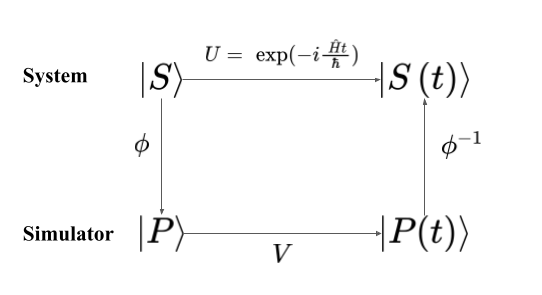
\includegraphics[width=\textwidth]{fig_10.png}}
\centering
\caption{$\ket{S}$ and $\ket{S(t)}$ represent the initial and final state (time evolved state) of system. Similarly, $\ket{P}$ and $\ket{P(t)}$ represent initial and final state of the simulator. }
\label{fig 10}
\end{figure}
Here the system is mapped to the simulator via an invertible map $\phi$ ( operator ). This mapping determines the correspondence between the states and operators of the system and simulator.\par
If we follow such a scheme described by figure $\ref*{fig 10}$, the evolution operator $U$ and $ V$ would be connected by,
\begin{equation}
V = \phi U \phi^{-1}
\end{equation}
If mapping is unitary, we can write,
\begin{equation}
V = e^{- i \hbar H_{sim} t}
\end{equation}
Where $H_{sim} = \phi H_{sys} \phi^{-1}$.\par
Thus while simulation we map the initial state $\ket{S}$ to $\ket{P}$
\begin{equation}
\ket{P} = \phi \ket{S} 
\end{equation}
Then simulator is allowed to time evolve $\ket{P} \xrightarrow{V} \ket{S}$. After time evolution final state $\ket{P(t)}$ is mapped back to $\ket{S(t)}$.
\begin{equation}
\ket{P(t)} = \phi^{-1}\ket{S(t)}
\end{equation}
Thus eventually we get back the time evolution of the system $\ket{S} \rightarrow \ket{S(t)}$.

Now we are going to discuss a very simple scheme of mapping between quantum system and simulator. The scheme we are discussing is proposed by Somaroo et al. (1999)\cite{somaroo} for simulating a quantum harmonic oscillator on two proton nuclear spins in 2,3-dibromothiophene. Note that here the number of states available for QHO is restricted to $4$. The convenient unitary mapping of system and simulator is,
\begin{gather*}
\ket{n=0} \leftrightarrow \ket{\uparrow\uparrow}
\ket{n=1} \leftrightarrow \ket{\uparrow\downarrow}
\ket{n=2} \leftrightarrow \ket{\downarrow\uparrow}
\ket{n=3} \leftrightarrow \ket{\downarrow\downarrow}
\end{gather*}
One doesn’t need to have followed this mapping. The mapping presented above is simple and straight forward. \par
The time evolution operator of QHO is given by
\begin{equation}
U = e^{-i\hbar H_{QHO} t} \equiv \exp\left[-i\left(\frac{1}{2}\ket{0}\bra{0} + \frac{3}{2}\ket{1}\bra{1} + \frac{5}{2}\ket{2}\bra{2} + \frac{7}{2}\ket{3}\bra{3}\right)\hbar\omega t\right]
\end{equation}
Where $\omega$ is the oscillatory frequency. From this, we can find the time evolution of the simulator.
\begin{equation}
\label{eq:19}
V = e^{-i\hbar H_{sim} t} \equiv \exp\left[-i\left(\frac{1}{2}\ket{\uparrow\uparrow}\bra{\uparrow\uparrow} + \frac{3}{2}\ket{\uparrow\downarrow}\bra{\uparrow\downarrow} + \frac{5}{2}\ket{\downarrow\uparrow}\bra{\downarrow\uparrow} + \frac{7}{2}\ket{\downarrow\downarrow}\bra{\downarrow\downarrow}\right)\hbar\omega t\right]
\end{equation}
In Pauli basis ${\sigma_{x},\sigma_{y},\sigma_{z},I}$, equation $\ref{eq:19}$ can be rewritten as ,
\begin{equation}
\label{eq:20}
V = exp\left[i\left(\sigma_{z}^{2}(1 + \frac{1}{2}\sigma_{z}^{2}) - 2 \right)\omega t\right]
\end{equation} 
Thus the simulator evolves according to equation $\ref{eq:20}$. At the end of the simulation, final state of the simulator is measured. The resultant state is mapped back into the QHO state.\par

Sometimes we can simulate not able to simulate the entire system. But mapping can be done in such a way that it could be used to study some characteristic of the system. In general, the mapping we use depends upon the characteristic of the system we intend to study and the properties of the simulator. In AQS the physical quantities can be measured directly from the simulator. Since it is analogous to the system, measurement results yield information about the system. This is an added advantage since in DQS we need to computationally manipulate the measurement results. Also in AQS even if there are we can use it to perform qualitative studies. But the error rate should be below a tolerance level. In such cases, AQS can be used to investigate properties like phase transition.  
 
Now in the example, we have shown, the mapping was simple and straight forward. But generally, this is not the case. Sometimes clever mapping schemes have to formulated to efficiently simulate a system. Further discussion in this direction can be seen in the reference \cite{georgescu}.

\section{ Quantum-information-inspired algorithms for classical simulation of quantum systems }
In this mode of approach, classical algorithms are used in the simulation of the quantum many body systems. But as discussed before, normal classical algorithms are prone to exponential explosion. Here in order to prevent this and to efficiently perform simulations we seek the assist of quantum information theory. First approach in this direction was done by Verstraete \emph{et al.}(2004), they analysed the Density Matrix Re-normalization Method from a quantum information perspective \cite{cirac}.\par This new hybrid class of algorithms help in efficient simulations of quantum lattice systems. Moreover, these methods can be combined with Monto Carlo Techniques to improve its efficiency. For example,it has been shown the quantum version of Metropolis alogarithm overcomes the sign problem that we discussed before \cite{temme2011}.

\bibliography{ref}
\printindex

\end{document}



\end{document}
